\documentclass[12pt]{article}
\usepackage[a4paper, margin=.30in]{geometry}
\usepackage{graphicx ,
            wrapfig,
            xcolor, 
            enumerate,
            amsmath,fontenc
            }

\newcommand\headerMe[2]{\noindent{}#1\hfill#2}
\renewcommand{\thesection}{\Roman{section}}

\author{Zakaria HAOUZAN}
\date{\today}

\begin{document}
% headers --------------
\headerMe{Matière : Physique-Chimie}{Professeur : Zakaria HAOUZAN}\\
\headerMe{Unité : Travail Mécanique et Energie }{Établissement : Lycée SKHOR qualifiant}\\
\headerMe{Niveau : 1BAC-SM-X}{Heure : 6H}\\

% ------Content ________
\begin{center}

    \Large{Leçon $N^{\circ} 6 $: \color{red}ENERGIE THERMIQUE ET
TRANSFERT THERMIQUE (Sc.Math) }
\end{center}

%\begin{wrapfigure}[10]{r}{0.5\textwidth}
%    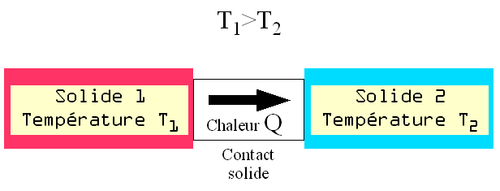
\includegraphics[width=0.5\textwidth]{./img/img00.png}
%\end{wrapfigure}
\section{Transfert thermique: }
\subsection{Définition et sens transfert thermique: }
Lorsque 2 corps à des températures différentes sont mis en contact, on constate que
la température du corps chaud diminue tandis que celle du corps froid augmente. Il y a
transfert d’énergie entre les deux corps : c’est le transfert thermique.
Un transfert thermique se fait spontanément du corps ayant la température la plus
élevée vers le corps ayant la température la plus basse.
\begin{center}

   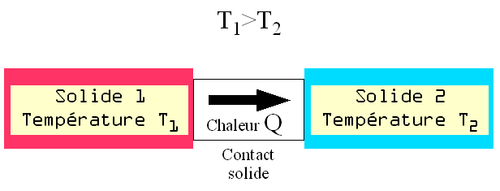
\includegraphics[width=0.5\textwidth]{./img/img00}
\end{center}

\subsection{Modes de transfert thermique: }
\subsubsection{transfert thermique par conduction:}
{Définition:} Transfert thermique par conduction est un mode de transfert d’énergie ayant lieu à
travers des corps conducteurs thermique sans déplacement de la matière

\subsubsection{transfert thermique par convection: }
{Définition:} Transfert thermique par convection est un autre mode de transfert d’énergie avec
déplacement de la matière

\subsubsection{Effets du transfert thermique:}

Le transfert peut élever la température d'un corps.

Le transfert thermique peut aboutir à un
changement d'état physique d'un corps pur.

\section{ Transfert thermique et Energie thermique:}
\subsection{Energie thermique (Quantité de chaleur): }

 {Définition:}Un transfert thermique est un transfert d'énergie d'un corps chaud (ou système chaud)
à un corps froid (ou système froid), cette énergie est dite énergie thermique (ou quantité de
chaleur). on note une énergie thermique par la lettre Q, son unité dans S.I. des unités est le
joule noté (J).
$$Q = m.C.(\theta_f - \theta_i)$$

Q : énergie thermique ou quantité de chaleur (J) 

m : masse (kg) , $\theta_i$ : température initiale (K)

C : capacité thermique massique ($J.kg^{-1}.K^{-1}$)
$\theta_f$: température finale (K) , 
\\Convention: Un système peut recevoir ou céder de l’énergie
par transfert thermique avec l'extérieur.
\begin{itemize}
        \item Si système reçoit effectivement de
l’énergie par transfert thermique, Q sera positive 
\item Si système perd effectivement de l’énergie
par transfert thermique, Q sera négative
\end{itemize}

\subsection{Définition capacité thermique massique C:}
La capacité thermique massique d'un corps pur est l'énergie thermique nécessaire à 1 kg de
ce corps pour élever sa température de 1°C.
\begin{center}
   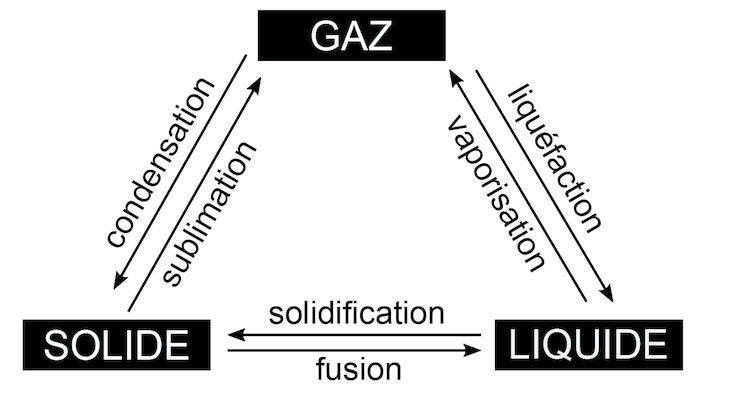
\includegraphics[width=0.5\textwidth]{./img/img01}
\end{center}

\subsection{Définition capacité thermique $\mu$:}
La capacité thermique $\mu$ d'un corps de masse m est l'énergie thermique nécessaire pour
élever sa température de 1°C, elle est exprimée par la relation:
$$\mu = m.C$$
$\mu :$ capacité thermique $(J.K^{-1} ) ou (J.C^{-1})$

m : masse (kg) ;

C : capacité thermique massique $(J.kg^{-1}.K^{-1})$
\\\underline{Remarque :}

La capacité thermique $\mu$ d'un système (S) formé de plusieurs corps est égale à la somme des
capacités thermiques de ces corps : $$\mu_s = \sum_i{\mu_i} = \sum_i{m_i.C_i}$$

\subsection{Equilibre thermique: }
Lorsque deux corps de températures différentes entrent en contact "dans une enceinte
isolante : fuites thermique négligeable", ils échangent de l’énergie thermique : le corps chaud
perd de l'énergie Q' et sa température diminue tandis que le corps froid perd de l'énergie Q et
sa température augmente.

Le transfert thermique se produit de sorte à ce que leurs températures respectives
s’égalisent. ils sont alors dans un état appelé équilibre thermique, il est exprimé par la
relation
$$Q + Q' = 0$$

Remarque :
Souvent un transfert thermique s'accompagne
de fuites thermiques pour remédier à ce problème
"minimiser les fuites" on utilise souvent une
enceinte adiabatique ( pas d'échange thermique
avec le milieu extérieur ) qui n'est autre que le
calorimètre.
\begin{center}

   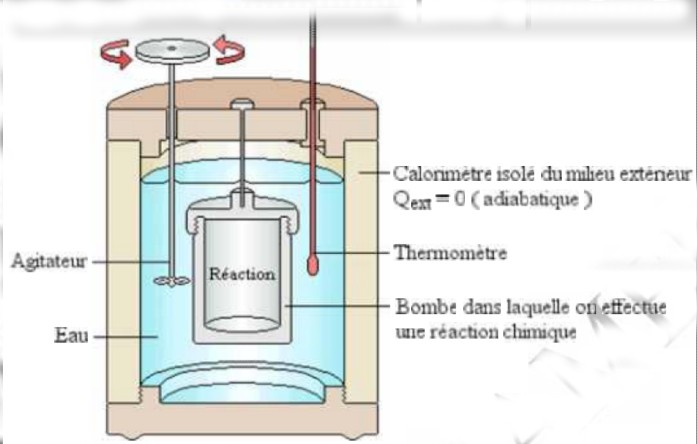
\includegraphics[width=0.5\textwidth]{./img/img02.jpg}
\end{center}

\section{Application 1 : Détermination de la capacité thermique d'un calorimètre }

La capacité thermique d'un calorimètre (et ces
accessoires) est l'énergie nécessaire pour élever la
température du calorimètre et ses accessoires de 1°C. on
la note $\mu_C$. 

On verse rapidement une masse m2 d'eau chaude de
température $\theta_2$ dans un calorimètre contenant une masse
m1 d'eau froid de température $\theta_1$. on agite le mélange,
après un moment la température du mélange se stabilise à
$\theta$ (équilibre thermique)

\begin{itemize}
    \item Le système (S) formé par le calorimètre et la masse m1 d'eau
reçoit une énergie Q1 $Q_1 > 0$
        $$Q_1 = m_1.C_e(\theta - \theta_1) + \mu_C(\theta - \theta_1)$$
    \item La masse m2 d'eau chaude perd une énergie Q2 $(Q_2 < 0)$
        $$Q_2 = m_2.C_e(\theta_2 - \theta) $$
    \item A l'équilibre thermique : $Q_1 + Q_2 = 0$  donc $$\mu_C = \frac{m_2.C_e.(\theta_2 - \theta)}{(\theta - \theta_1)} - m_1.C_e$$
\end{itemize}
\section{Application 2 : Détermination de la capacité thermique massique d'un métal : }

On dispose d'un calorimètre de capacité thermique $\mu_C$ contenant une masse $m_1$ d'eau dont la température est $\theta_1$.

On introduit dans le calorimètre un petit bloc d'un métal de masse m après buillante et l'avoir séché.

après agitation la température du mélange se stabilise à $\theta$

$m_1 = 300g$ et $m = 122g$ , $\mu_C = 100J.K^{-1}$ , $\theta_1 = 19.8 ^\circ{C}$ $\theta_2 = 22.1 ^\circ{C}$

\begin{itemize}
        \item Le système (S1) formé par le calorimètre et la masse m1 d'eau
reçoit une énergie Q1 $Q_1 > 0$ $$Q_1 = m_1.C_e(\theta - \theta_1) + \mu_C(\theta - \theta_1)$$
\item Le système (S2) formé par le bloc de métal a perd une énergie Q2 $(Q2 < 0)$:
    $$Q_2 = m.C(\theta - \theta_2)$$
        \item A l'équilibre thermique entre les 2 systèmes : Q + Q = 0 
            $$C = \frac{(m_1.C_e + \mu_C)(\theta - \theta_1)}{m.(\theta_2 - \theta)}$$
\end{itemize}

\section{Exercice d'application N°1:}
On verse rapidement dans un calorimetre de capacité thermique $\mu_C = 210 J.C^{-1}$
une
masse m1 = 355 g d'eau dont la température $\theta_1$ = 23,8 °C. on introduit ensuite dans le
calorimètre un morceau de laiton " alliage composé essentiellement de cuivre et de zinc "
de masse m2 = 173 g et de température $\theta_2$ = 88,5 °C.

1) Comment appelle-t-on le transfert d'énergie entre les 2 systèmes {calorimetre , masse d'eau} et {morceau de laiton} . 

2) Préciser le sens du transfert.

3) Ecrire la relation traduisant l'équilibre thermique ayant lieu.

4) en déduire la température finale q du mélange sachant que la capacité thermique
massique du laiton est C = 378 $J.kg^{-1}.C^{-1}$

\section{Transfert thermique avec changement d'état physique d'un corps pur (chaleur latente) : }
\begin{center}

   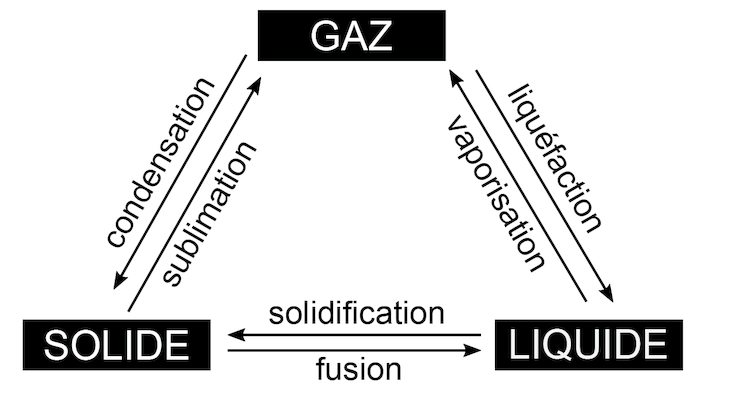
\includegraphics[width=0.5\textwidth]{./img/img01.jpg}
\end{center}




\subsection{Chaleur latente massique de fusion $L_f$ : }

La chaleur latente massique $L_f$ de fusion d'un corps pur est l'énergie thermique
nécessaire pour transformer totalement à 1 kg de ce corps de l'état solide à l'état
liquide à température $\theta_f$ et pression constant

\underline{\textbf{Expression de l'énergie thermique : }}L'énergie reçue par le corps pur au cours de sa fusion, à température et pression
constante, est donnée par la relation : $$Q = m.L_f$$
Q : énergie thermique (J) , m : masse (kg) ; Lf : Chaleur latente massique de fusion $(J.kg^{-1})$
\begin{center}
\begin{tabular}{|c|c|c|}
    \hline
    Corps pur &$L_f(j.kg^{-1})$ &$\theta_f(^{\circ}C)$\\\hline
    Glace     & $3.35.10^5$ & 0 \\\hline
    Aluminium & $4.04.10^5$ & 660\\\hline
    Fer       & $2.70.10^5$ & 1635\\\hline
    \end{tabular}
\end{center}
Remarque :
On admet que l'énergie Q' perdu par le corps pur au cours de sa solidification, à
température et pression constante, est : Q' $= m × L_{sol}$ ; Q'$<$ 0  avec $L_{SOL}$ Chaleur
latente massique de solidification ; avec Q'=Q  donc : $L_{SOL} = -L_f$

\subsection{Exercice d'application N°2:}
Cent tonnes de ferrailles sont chauffées dans un four électrique afin d'obtenir du fer
liquide à 1538°C. La température initiale est 20°C. La durée de l'opération dure 5 heures
et le rendement du four est de 70\%.
Données : 

$C_fer = 450 J.kg^{-1}K^{-1}$ ; $L_{fusion fer}= 270 kJ.kg^{-1} ; \theta_{f(fer)} = 1538$°C. Quelle est l'énergie électrique nécessaire. En déduire la puissance du four.

\subsection{Vaporisation et liquéfaction :}
Définition Chaleur latente massique de vaporisation $L_V$:
La chaleur latente massique $L_V$ de fusion d'un corps pur est l'énergie thermique
nécessaire pour transformer totalement à 1 kg de ce corps de l'état liquide à l'état
gazeux à température $\theta_V$ et pression constante.

L'énergie reçue par le corps pur au cours de sa vaporisation, à température et
pression constante, est donnée par la relation :
$$Q = m.L_V$$
Q : énergie thermique (J.) ; m : masse (kg) ; $L_V$ : Chaleur latente massique de vaporisation ($J.kg^{-1}$)
\begin{center}
\begin{tabular}{|c|c|c|}
    \hline
    Corps pur     &$L_V(Kj.kg^{-1})$ &$\theta_V$\\\hline
    eau           & $2261$  & 100 \\\hline
    éthanol       &  $906$  & 78\\\hline
    dioxygène     & $212.5$ & -182.962\\\hline
    dihydrogene   & $450$   & -252.87\\\hline
    \end{tabular}
\end{center}

Remarque :
On admet que l'énergie Q' perdu par le corps pur au cours de sa liquéfaction, à
température et pression constante, est :Q' = m × L ; Q'$<$ 0 avec $L_l$ avec $L_l$ Chaleur
latente massique de liquéfaction; avec Q' = -Q donc : $L_l = -L_V$
\begin{center}

   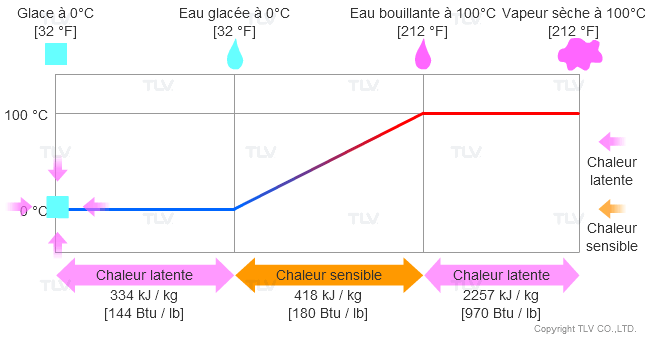
\includegraphics[width=0.8\textwidth]{./img/img02-1.png}
\end{center}

\section{Transfert d’énergie par rayonnement: }
L'énergie transportée sous forme de radiations
électromagnétiques est appelée énergie rayonnante.
Elle est notée WR. Elle s'exprime en Joule. Tout
corps chaud émet des radiations électromagnétiques
qui transportent de l'énergie.

\section{Energie interne et transfert d’énergie:}
\begin{itemize}
      \item  Si le transfert s'effectue par travail uniquement, la variation de l'énergie interne du
système est : $\Delta{U} = W$ avec W étant l'énergie transfert par travail
\item Si le transfert s'effectue seulement par chaleur, la variation de l'énergie interne du
système est : $\Delta{U} = Q$  Avec Q étant l'énergie transfert par chaleur
\item Si le transfert s'effectue par travail, par chaleur ou par rayonnement, la variation de
l'énergie interne du système est :  $\Delta{U} = W + Q_T$  Avec Q étant l'énergie transfert par chaleur et/ ou par rayonnement

\end{itemize}
\end{document}

